\chapter{Design}

This section goes over the initial design for the solution we present. Any major deviations from this design are noted in Chapter~\ref{chap:Deviations}. To make design decisions, we re-evaluate the functional requirements taking into account the techniques gleaned and the lessons learnt from Background and Related Work

\section{Static vs Dynamic}

The first and largest choice faced is whether to use dynamic or static detouring for our library. After deciding this, we can evaluate the available implementation options.

Even though implementing detouring at runtime offers advantages such as flexibility and ease of development, it was ruled out as an option because we did not find a dynamic method which does not compromise \emph{(F6)}. That is, all the runtime methods we have looked at require some form of environment, whether this is through the distribution of a shared library, process-level virtual machine or otherwise. Since a dynamic solution is infeasible, we can narrow the scope of the solution to the various static binary rewriting approaches.

We propose a library which will enable the user to rewrite a binary 

\begin{figure}[H]
 \centering
 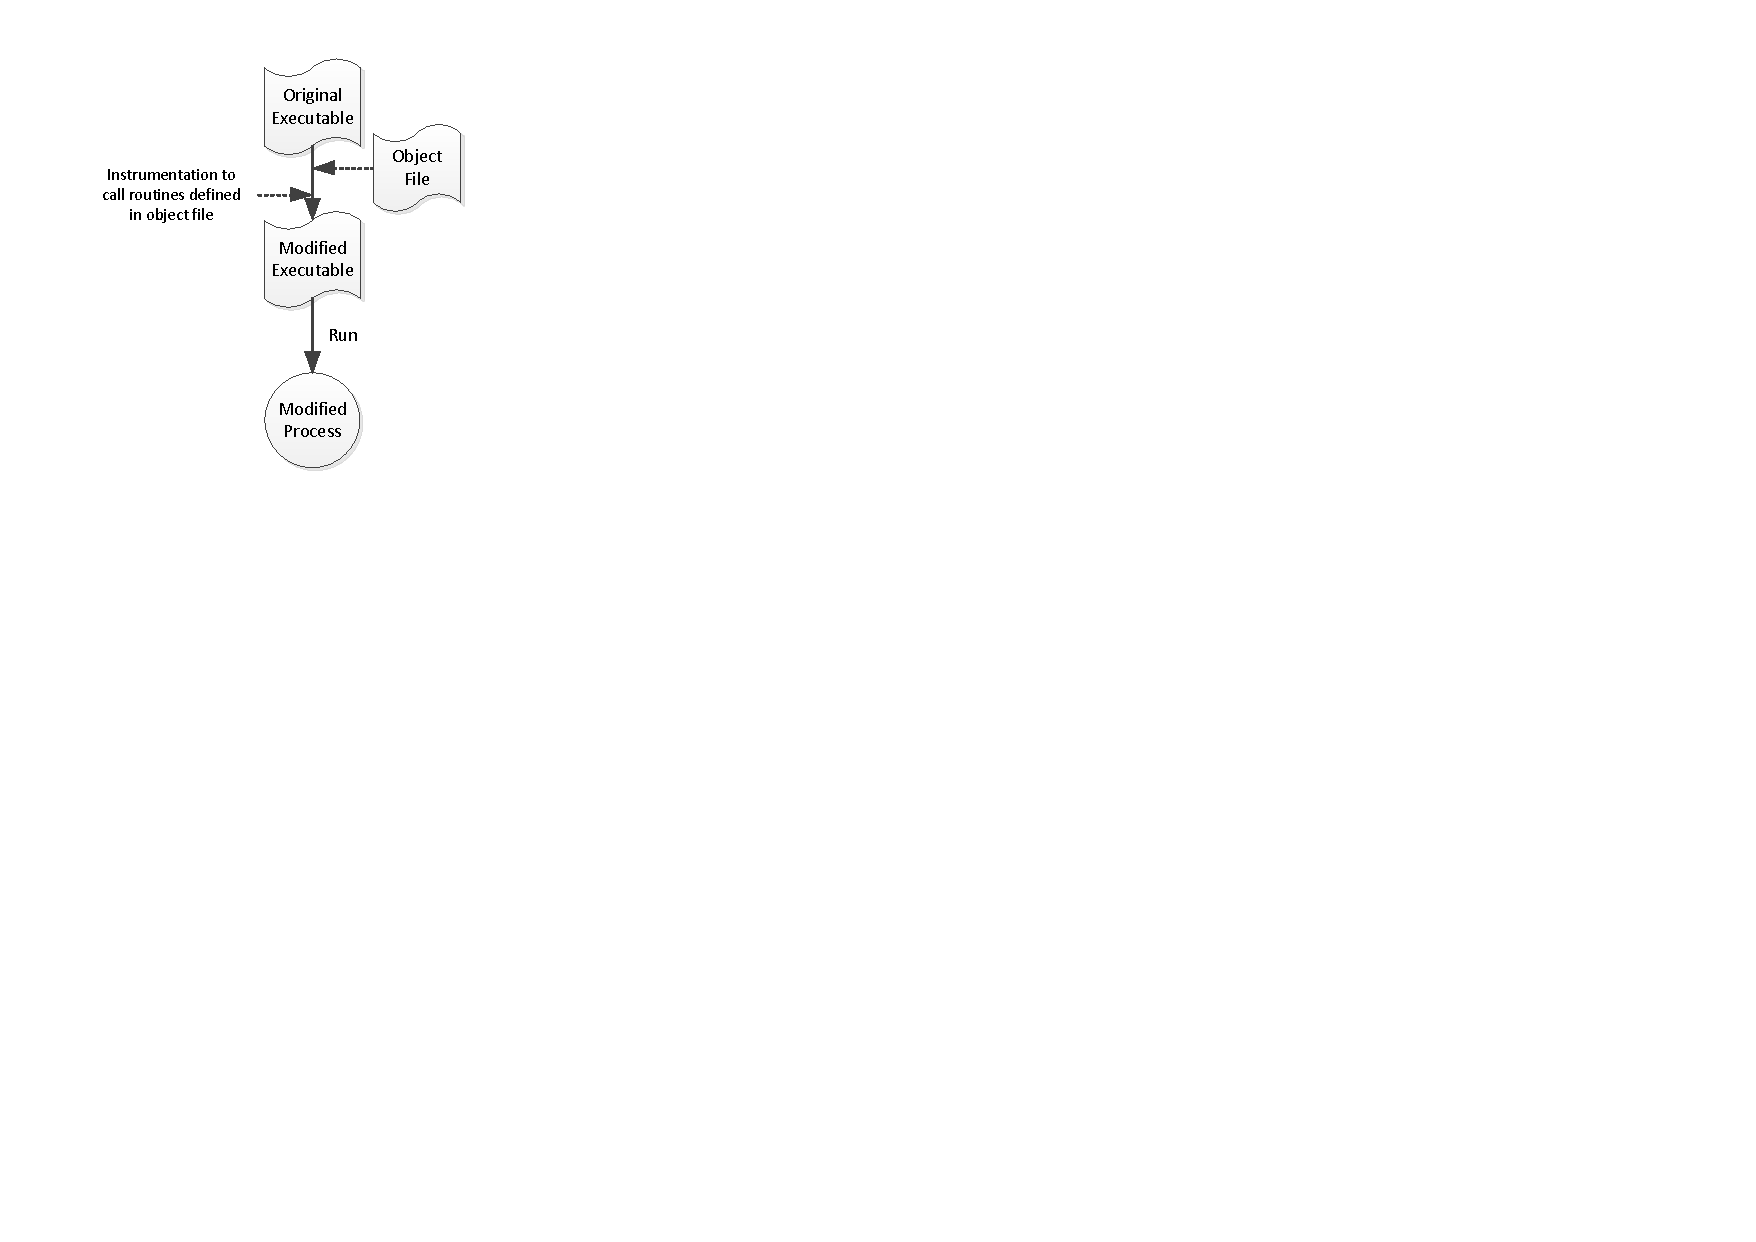
\includegraphics{Workflow.pdf}
 \caption[Hierarchy]{The proposed method for instrumentation. An object file containing user defined routines is optionally injected into the target binary. Using binary rewriting, the original code is then connected to the injected code.}
\end{figure}



We propose an implementation of executable editing which works on top of the BFD library. This makes adaquate use of existing functionality as required by \emph{(F7)}. BFD will work in conjunction with the opcodes library to produce the control flow graph as required by \emph{(F4)} and \emph{(F5)}. To inject user-defined routines, we can take a similar approach to EEL and allow the user to specify an object file to be merged with the target binary. The next step would then be to find some mechanism by which procedural-level detouring can be achieved \emph{(F1)}. This is the first point at which we are modifying the target's code in any way. The technique used will have to be modified slightly to accommodate for the trampolining as required by \emph{(F2)}. Since the user defined functions are compiled separately to the target, they do not know what address to call for the trampoline so this is something we will have to deal with.